%\documentclass[twoside,hidelinks]{ctuthesis}
\documentclass[twoside]{ctuthesis}
\usepackage{hyperref}

\ctusetup{
xdoctype = B,
xfaculty = F3,
mainlanguage = english,
titlelanguage = english,
title-english = {Application for personal development},
title-czech = {Aplikace pro podporu osobního rozvoje},
keywords-english = {word, key},
keywords-czech = {slovo, klíč},
author = {Artem Vanyukhin},
supervisor = {Ing. Pavel Náplava, Ph.D.},
fieldofstudy-english = {Software Engineering and Technology},
day = 1,
month = 5,
year = 2021,
}

\ctuprocess

\begin{thanks}
    Thanks\ldots
\end{thanks}

\begin{declaration}
    I  hereby  declare\ldots

    In Prague on \monthinlanguage{title} \ctufield{day}, \ctufield{year}
\end{declaration}

\begin{abstract-english}
    The purpose\ldots
\end{abstract-english}

\begin{abstract-czech}
    Cíl\ldots
\end{abstract-czech}

\begin{document}

    \maketitle
    %!TEX ROOT=main.tex

\chapter{Introduction}\label{ch:introduction}

%//IDEA Friendly competition

This chapter will introduce the reader to author's motivation, problem description and the basic idea of the future application.

~\nameref{sec:introduction-motivation} section describes personal point of view of the author.
Detailed analysis of the related domain will be the part of ~\nameref{ch:personal-development-domain} chapter.

~\nameref{sec:problem-description} section describes problems application will attempt to solve and
~\nameref{sec:solution-idea} section will draw basic idea of the application, whereas exact approach
will be introduced in following chapters: ~\nameref{ch:solution-analysis}, ~\nameref{ch:implementation}, ~\nameref{ch:testing}.


\section{Motivation}\label{sec:introduction-motivation}

{\color{gray}//ASK Can I write here from my perspective?}

From an elementary school till the final year of university studies, one was able to compare himself to peers.
This could be the source of strong motivation that stimulates continuous process of learning.
In order to keep myself from falling into daily routine of work when my studies are over,
but instead to continue to actively study, I decided to look into applications for personal development.
Prompt research showed that there is a lack of applications that could provide strong social engagement features
as well as be helpful without them.

Applications with social engagement elements seems to be well accepted by users.
Those that exists lack crucial functionalities that could help the process and aim exclusively to the competition idea.
This paper will shortly examine the domain of personal development, compare existing solutions and provide an analysis for a
new application.
{\color{gray}//ASK Mention implementation here?}

\section{Problem description}\label{sec:problem-description}

Personal development is a life-long process.
As well as many other activities, this process is more effective with defined, measured approach.
There are many well-build solutions aimed to structure process of personal development.
These solutions have variety of ways to approach their users, which means that each could find an application that works for them.
The problem with these applications is small to none amount of social engagement.
Users should be motivated and disciplined enough in order to use such application for a long time.

Another type of personal development applications are habit trackers.
These applications aimed at development of new desired habits and abandonment of unwanted.
Habit trackers often include gamification elements and usually there is a slight social engagement element.
On the other hand, these applications usually lack more structural approach, visual reports and planning features.

Application that motivate user through interaction with others and capable of activity planning and data visualisation
will take the best from both application types mentioned above and provide better user experience.
The problem of this paper is analysis and proposal ~{\color{gray}//ASK and implementation?} of such application.

\section{Solution idea}\label{sec:solution-idea}

bla
    %!TEX ROOT=main.tex

\chapter{Personal development domain}\label{ch:personal-development-domain}


This section will introduce the reader to the domain of personal development.
Justification of the idea behind the application will also be presented here.

%Use empirical statements
\section{Definition of personal development}\label{sec:definition-of-personal-development}

In order to create helpful application, it is crucial to build it based on principles and ideas of personal development.
Familiarization with these will start from the definition of personal development and with Maslow's hierarchy of needs in particular.

\begin{figure}[h]
    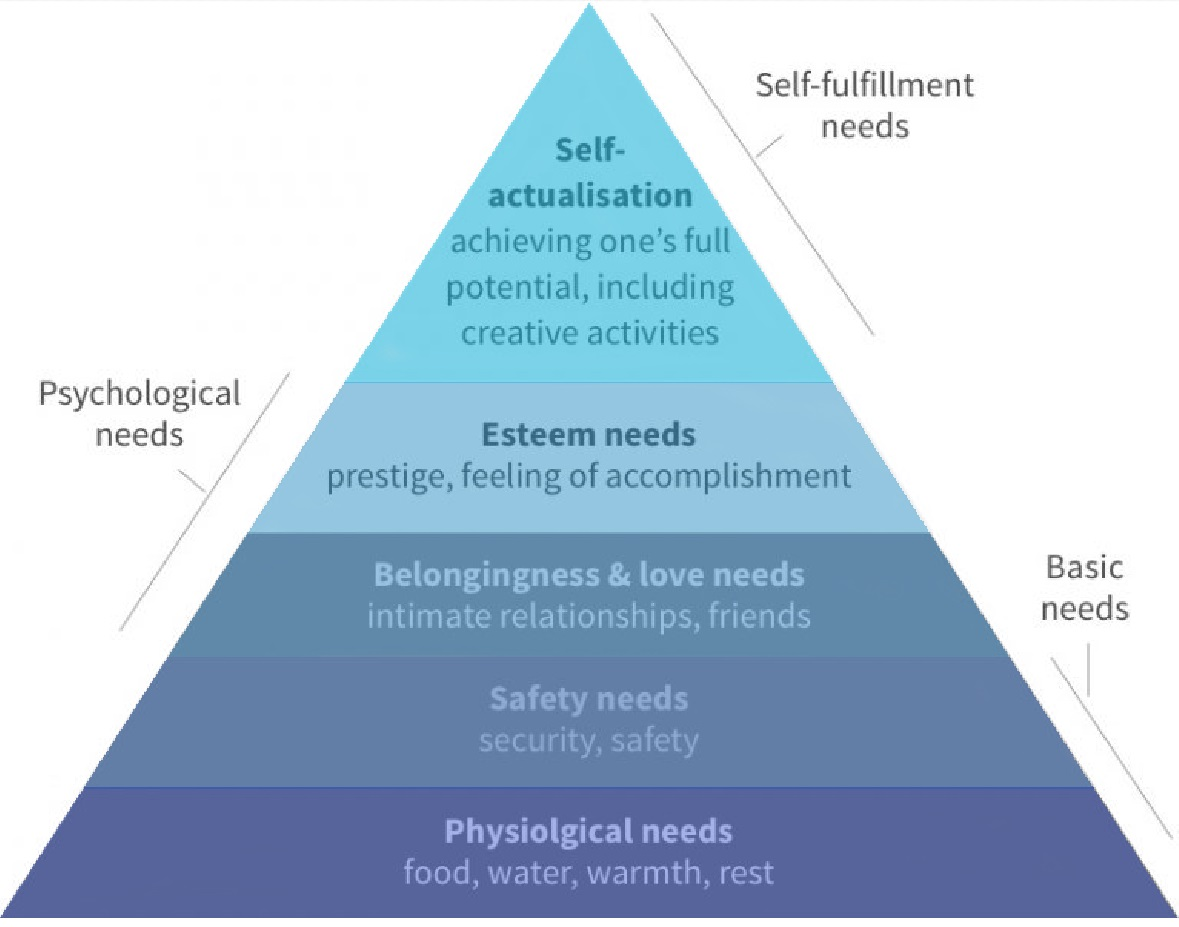
\includegraphics[width=0.75\textwidth]{images/maslows.jpg}
    \caption{Maslow's Hierarchy of Needs~\cite{maslows}}
    \label{fig:maslows}
\end{figure}




It is fair to say, that each person could give own definition of personal development.
It is nesse
It requires no special knowledge to define what personal development is.

Every person is aware of the concept of personal development.
The process of personal development is natural.

    %!TEX ROOT=main.tex

\chapter{Existing solutions}\label{ch:existing-solutions}

This section will introduce the reader to the analysis of existing applications.

%Comparison criteria
%!TEX ROOT=main.tex

\section{Comparison criteria}\label{sec:comparison-criteria}

%https://play.google.com/store/apps/details?id=com.habitfactor&hl=en

%https://play.google.com/store/apps/details?id=com.remente.app&hl=en

Based on previous chapter, core features for the application are following: personal development planning and social engagement.
Application also has be cross-platform.

\textit{Personal development planning} encapsulates features that application provides for structurized approach to personal development.
This should handle repetitive activities as well as long-term plans.
Progress tracking and ability to review old plans are also a part of this criteria.

\textit{Social engagement} criteria includes features that application provide for interaction between users.
It might be goal progress sharing or common goals that users pursue at the same time.

\textit{Multiplatform} is another crucial criteria.
%TODO improve justification for multiplatform criteria
Only web, Android and iOS platforms are considered in terms of this project.
Windows, Macintosh and Linux are not going to be considered due to decrease of popularity of desktop platform.\cite{mobile-vs-desktop}



%Data collection
%!TEX ROOT=main.tex

\section{Data collection}\label{sec:data-collection}

Data collection was done using Google search engine as it was the most popular search engine in 2020 with over 90\% market share.\cite{google-market-share}
The first step was to find applications using following keywords: "personal development apps", "habit tracker", "self-improvement apps".
The top five results for each keyword were used to gain the initial dataset.
The next step was to manually filter gathered data.
The first step of filtration was to manually remove duplicates.
The second step was to remove activity specific applications: sport, meditation, brain training.
The third step was to remove applications with static textual content on topics of psychology, personal development and life improvement techniques.
The fourth step was to remove applications aimed exclusively at personal care, skincare, mood journals and sleep journals.
The fifth step was to remove business and productivity applications aimed primarily at small scale time management, short-term goals and daily productivity.
The sixth step was to remove applications aimed strongly at bad habit breaking, such as smoking and drinking.
The seventh step was to remove applications available for single platform exclusively, e.g., iOS\@.
The final step was to remove applications that are very similar in terms of interface, user experience and functionality.

\begin{table}[t!]
    \centering
    \begin{adjustbox}{width=\textwidth}
        \begin{ctucolortab}
            \begin{tabular}{llllll}
                \bfseries Action & \bfseries K1 & \bfseries K2 & \bfseries K3 & \bfseries Total results & \bfseries Difference \\\Midrule
                Initial dataset & 52 & 38 & 62  & 152 & +152\\
                Duplicates & 46 & 25 & 23  & 94 & -58\\
                Sport oriented & 41 & 23 & 22  & 86 & -8\\
                Meditation oriented & 38 & 19 & 19  & 76 & -10\\
                Brain training oriented & 25 & 16 & 18  & 59 & -17\\
                Topics oriented & 15 & 16 & 10  & 41 & -18\\
                Personal care oriented & 5 & 11 & 7  & 23 & -18\\
                Business and productivity oriented & 4 & 11 & 5  & 20 & -3\\
                Bad habits oriented & 4 & 10 & 1  & 15 & -5\\
                Single platform & 2 & 5 & 1  & 8 & -7\\
                Similar applications & 2 & 2 & 1  & 5 & -3\\
                \bottomrule
                \multicolumn{6}{1}{K1="Personal development apps", K2="Habit tracker", K3="Self-improvement apps"}
            \end{tabular}
        \end{ctucolortab}
    \end{adjustbox}
    \caption{Dataset filtering}
    \label{tab:dataset-filtering}
\end{table}

The result of filtering is 5 applications that will be analyzed in the next section.
Details of the dataset filtering process are described in Table~\ref{tab:dataset-filtering}.
\textit{Action} column contains the removal criteria during a filtration step.
\textit{K1} to \textit{K3} columns contain the amount of applications by a keyword.
\textit{Total results} column contains the sum of K1, K2 and K3 columns.
\textit{Difference} column contains the difference of total results against previous row.

%Data analysis
%!TEX ROOT=main.tex

\section{Data analysis}\label{sec:data-analysis}

Following 7 applications will be analyzed in this section: Uloo.me, Habitica, Habitify, TickTick, Habitshare, Remente and Coach.me.
%
%\section{Uloo.me}\label{sec:uloo.me}
%
%\renewcommand{\arraystretch}{1.5}% Vertically stretch tabular constructions
%\noindent
%\begin{tabularx}{\textwidth}{
%@{\hspace{1.5em}}% Space for left bullet
%>{\leavevmode\llap{\textbullet~}\raggedright}% Left bullet + formatting of column
%X% Left column specification
%@{\quad\hspace{1.5em}}% Space between columns + right bullet space
%>{\leavevmode\llap{\textbullet~}\raggedright\arraybackslash}% Right bullet + formatting of column
%X% Right column specification
%@{}% No column space on right
%}
%    \toprule
%    \multicolumn{1}{X}{\centering\bfseries Pros} &
%    \multicolumn{1}{X}{\centering\bfseries Cons} \\
%    \midrule
%    One &
%    Two \\
%    \fakeleft &
%    Three \\
%    Four &
%    Five \\
%    \bottomrule
%\end{tabularx}
%
%In summary ...




%Conclusion
%!TEX ROOT=main.tex

\section{Conclusion}\label{sec:conclusion}

As the research showed, there is a variety of applications suited for tracking of long-term or repetitive activities.
Only TickTick proved to be suited for both, but not without its drawbacks.

Social engagement was efficiently utilized in Habitify and Habitica,
but those applications lack ability to track anything other than habits.

In conclusion, there is a visible gap that could be filled with even more social application that will provide
features for long-term and repetitive activities tracking.
    %!TEX ROOT=main.tex

\chapter{Solution analysis}\label{ch:solution-analysis}

This chapter will draw a solution analysis for the future application.
Based on the previous chapters there will be introduced entities of the domain and their lifecycle.
Later there will be description of functional requirements.

%Overall description
%!TEX ROOT=main.tex

\section{Domain model}\label{sec:domain-model}

This section will describe entities of an application domain model in details.

\subsection{User}\label{subsec:user}

User entity consists of a minimum required attributes in order to simplify registration process for end-user.
Recursive relation represents friendship between users, which is required for activity sharing.
Goal plans, goals and habits are always owned by one user and might be shared with many users.
Sharing is used for displaying private plans, goals and habits with specific users.

\subsection{Goal plan}\label{subsec:goal-plan}

Goal plan serves as a blueprint for a goal.
This separation of plan and goal allows users create and share not only their progress, but also plans themselves.
Possible use case would be the following.
A user is proficient in specific field or skill that other users would like to learn or gain.
They create a goal plan with tasks that contains instructions and share it with any amount of users.
Other users then able to start goal pursuing process using this shared plan.

\subsection{Goal}\label{subsec:goal}

Goal is a tool for pursuing and progress tracking of a long-term target.
It is also a specific case of fulfilling a goal plan that is created by user or shared with them.




%Domain model
%!TEX ROOT=main.tex

\section{Domain model}\label{sec:domain-model}

This section will describe entities of the application domain model displayed in figure below.
Some technical information, like data types, are omitted for brevity.
Each entity has information about creation date, modification date etc.

\begin{figure}[h]
    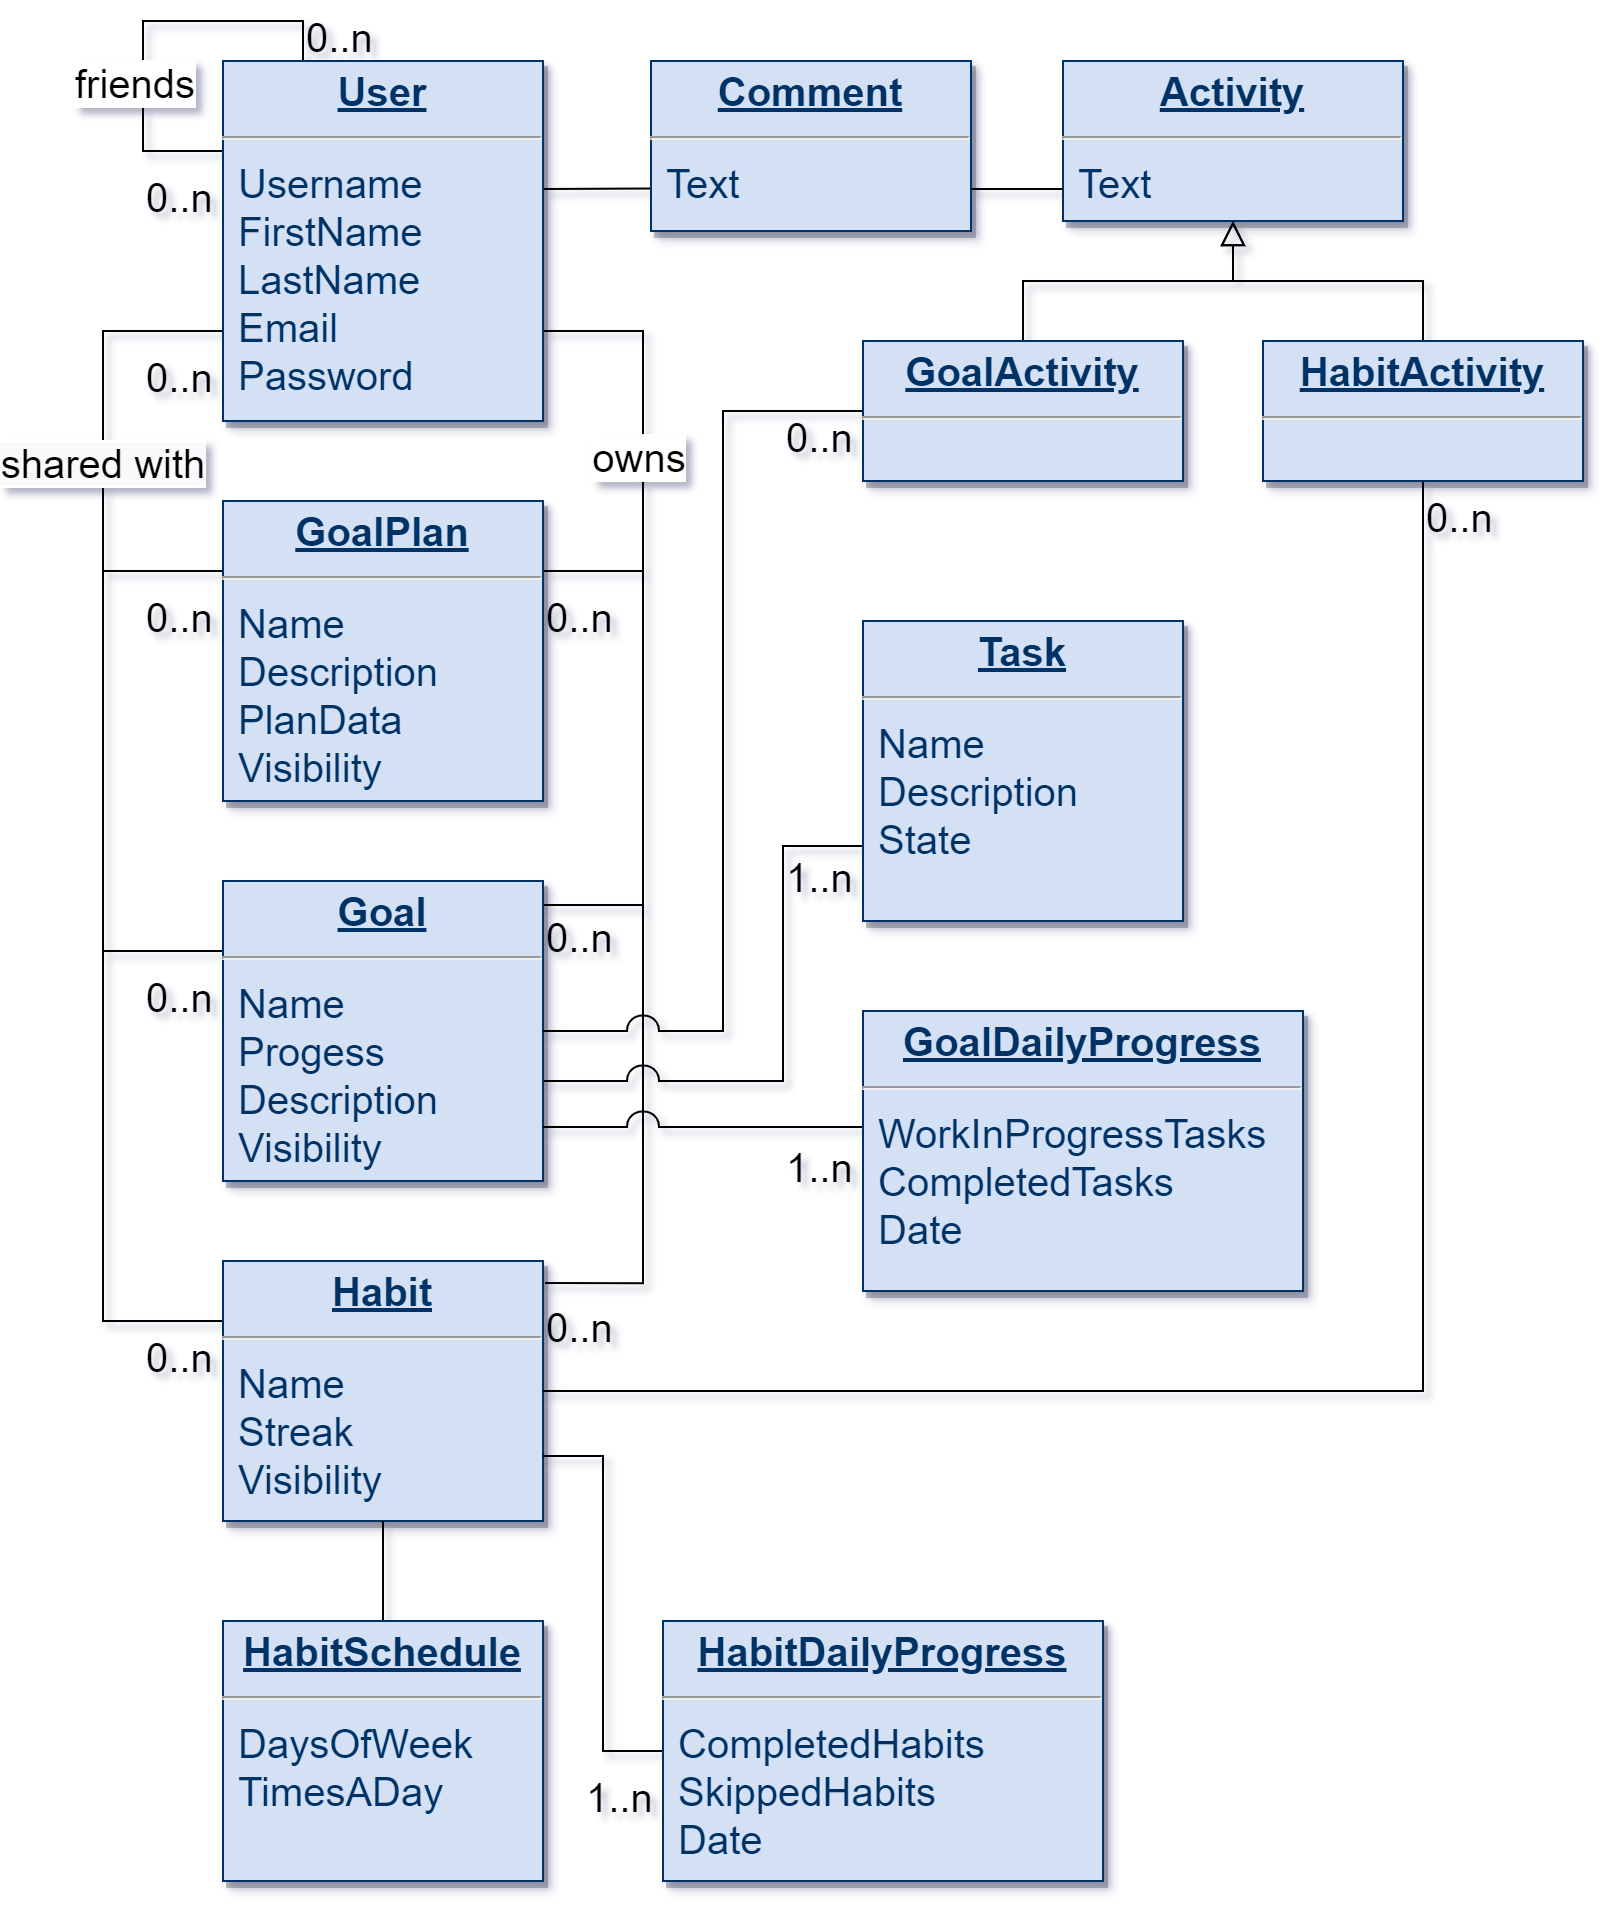
\includegraphics[width=0.75\textwidth]{images/pda-domain-model.png}
    \caption{Domain model}
    \label{fig:domain-model}
\end{figure}


\subsection{User}\label{subsec:user}

User entity consists of a minimum required attributes in order to simplify registration process for end-user.
Recursive relation represents friendship between users, which is required for activity sharing.
Goal plans, goals and habits are always owned by one user and might be shared with many users.
Sharing is used for displaying private plans, goals and habits with specific users.

\subsection{Goal plan}\label{subsec:goal-plan}

Goal plan serves as a blueprint for a goal.
This separation of a plan and a goal allows users to create and to share not only their progress, but also plans themselves.
Possible use case would be the following: a user is proficient in a specific field or skill that other users would like to learn or gain.
They create a goal plan with tasks that contains instructions and share it with any amount of users.
Other users then able to start goal pursuing process using this shared plan.

\subsection{Goal}\label{subsec:goal}

Goal is a tool for managing long-term targets.
It is also a specific case of fulfilling a goal plan that is created by user or shared with them.

\subsection{Task}\label{subsec:task}

Task is a building block of a goal.
Task completion used for calculation of a goal's progress.

\subsection{Goal daily progress}\label{subsec:goal-daily-progess}

This entity holds data about daily progress on a specific goal during given day.
It is then used for statistics calculation.

\subsection{Habit}\label{subsec:habit}

Habit is a tool for managing simple and repetitive targets.

\subsection{Habit schedule}\label{subsec:habit-schedule}

Each habit has a schedule.
At first it filled with default values, but it is possible for users to change them.

\subsection{Habit daily progress}\label{subsec:habit-daily-progress}

This entity holds data about daily progress on a specific habit.
It is then used for statistics calculation.

\subsection{Activity}\label{subsec:activity}

This entity holds data about user activities on goals and habits.
When goal or habit shared with user, they will see related activities.

\subsection{Comment}\label{subsec:comment}

It is possible to comment activities in application and reply to commentaries.
Everyone who has access to an activity can see all the commentaries.

%Functional requirements
%!TEX ROOT=main.tex

\section{Functional requirements}\label{sec:functional-requirements}

This section will introduce requirements regarding the application functionalities.

Requirements have their priority estimation.
High priority feature is a "must have" and necessarily needed in the application.
Medium priority feature is a "nice to have" and should be implemented for the best user experience.
Low priority feature is a "might have" which takes user experience level even further.

Complexity estimation is relative.
Medium might be considered as average time to implement a feature.
Low complexity level requirements takes noticeably shorter period of time to implement them.
High complexity level requirements as the opposite will take longer period of time.

\subsection{User registration and login}\label{subsec:user-registration-and-login}
\textbf{Complexity:} High\\
\textbf{Priority:} High\\
\textbf{Description:} In order to safely store and access data in the cloud, user needs registration and login features.\\
\textbf{Note:} This requirement brings the need for thorough security configuration.\\


\subsection{User login with a facebook account}\label{subsec:user-login-with-facebook-account}
\textbf{Complexity:} High\\
\textbf{Priority:} Medium\\
\textbf{Description:} Login through a Facebook account needed to minimize registration effort for a user.\\
\textbf{Note:} Meeting the Facebook's security criteria might take additional effort.\\


\subsection{Friend list}\label{subsec:friend-list}
\textbf{Complexity:} Low\\
\textbf{Priority:} High\\
\textbf{Description:} Users need the ability to add each other to friend lists in order to share activities with each other.\\


\subsection{Application is usable without a registration}\label{subsec:application-is-usable-without-registration}
\textbf{Complexity:} High\\
\textbf{Priority:} Low\\
\textbf{Description:} Ability to try the application without a registration improves experience for a user.\\
\textbf{Note:} This requirement will take large amount of time for analysis and will increase overall complexity of the system.\\


\subsection{Habits management}\label{subsec:habits-management}
\textbf{Complexity:} Medium\\
\textbf{Priority:} High\\
\textbf{Description:} Users need an interface to manage their repetitive activities.\\


\subsection{Goals management}\label{subsec:goals-management}
\textbf{Complexity:} Medium\\
\textbf{Priority:} High\\
\textbf{Description:} Users need an interface to manager their long-term goals.\\


\subsection{Goals planning}\label{subsec:goals-planning}
\textbf{Complexity:} Medium\\
\textbf{Priority:} High\\
\textbf{Description:} Users need an interface to create and share goal plans.\\


\subsection{Visibility of habit, goal, goal plan}\label{subsec:visibility-for-habit-goal-goal-plan}
\textbf{Complexity:} Medium\\
\textbf{Priority:} High\\
\textbf{Description:} Users need an ability to change visibility of their data.
There will be three levels of visibility: private, selected friends only, all friends.\\


\subsection{Activity history}\label{subsec:activity-history}
\textbf{Complexity:} Medium\\
\textbf{Priority:} High\\
\textbf{Description:} Users need an interface to see their activities on goals and plans.\\


\subsection{Activity sharing}\label{subsec:activity-sharing}
\textbf{Complexity:} High\\
\textbf{Priority:} Medium\\
\textbf{Description:} Users need an interface to see activities of other users.\\
\textbf{Note:} This requirement brings the need for visibility management of goals and habits between users.\\


\subsection{Basic statistics display}\label{subsec:basic-statistic-display}
\textbf{Complexity:} Medium\\
\textbf{Priority:} Medium\\
\textbf{Description:} Users need an interface to see their statistics of following habits and fulfilling goals.\\


\subsection{Gamification elements by activity points}\label{subsec:gamification-elements-by-activity-points}
\textbf{Complexity:} Low\\
\textbf{Priority:} Low\\
\textbf{Description:} Each finished activity related to habit gives user one point.
Activity points displayed in user profile.\\

%%High-level design
%%!TEX ROOT=main.tex

\section{Software architecture}\label{sec:software-architecture}

\begin{figure}[h!]
    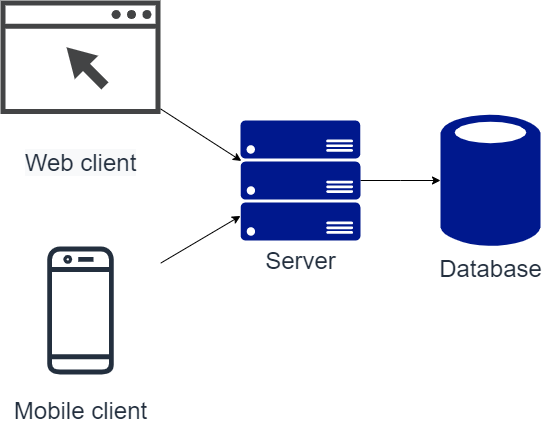
\includegraphics[width=0.75\textwidth]{images/high-level-architecture}
    \caption{High-level software architecture}
    \label{fig:high-level-architecture}
\end{figure}

Software architecture has been proposed with scalability and multiple types of client applications in mind.
As shown in figure~\ref{fig:high-level-architecture}, server is a standalone application separated from client applications.
Such separation allows sharing business logic across different client applications without a need of rewrite.
Another benefit is the simplicity of scaling.
New instance of the server application might be deployed behind load balancer as needed.

More specifically application is built using Model-View-Controller (MVC) architecture.\cite{wiki-mvc}
View component in MVC is a representational layer.
User interacts with the application through mentioned layer.
In case of this application View component is represented by client applications.
Model component represents business logic and Controller serves to bind View and Model.
Model and Controller components are encapsulated in server part of this application.

\begin{figure}[h!]
    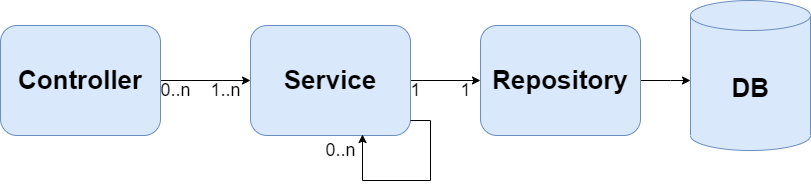
\includegraphics[width=1\textwidth]{images/server-mvc-spring}
    \caption{Server architecture}
    \label{fig:server-mvc-spring}
\end{figure}

Detailed server architecture displayed in figure 4.3.
Repository serves as a Data Access Object (DAO).
Each DAO defines the set of allowed operations over a specific entity of the domain model.
Service is an implementation of business logic.
Each Service has exactly one related Repository.
Other entities Repositories should be accessed via their Service component, hence 0-to-n cardinality from Service to Service.
Complex business logic scenarios with several Service components calls might be encapsulated using the facade design pattern.
Controller creates API endpoint mapping, e.g.\ in www.domain.com/users '/users' is an endpoint mapping.

Described architecture is supported out of the box by major web development frameworks as Spring (Java/Kotlin), Django (Python), Rails (Ruby).\cite{spring,django,ruby} etc.
This, alongside with preservation of the single-responsibility principle~\cite{wiki-srp} enforced by the idea of MVC, allows for rapid development of maintainable applications.
    %!TEX ROOT=main.tex

\chapter{Testing}\label{ch:testing}
    %!TEX ROOT=main.tex

\chapter{Testing}\label{ch:testing}
    %!TEX ROOT=main.tex

\chapter{Conclusion}\label{ch:conclusion}

The domain research provided an understanding of personal development process.
This understanding allowed proposition of data management.
The second part of the domain research justified that competitiveness might be used as a motivator for personal development.

Analysis of existing solution allowed spotting common pitfalls and gave ideas for features that might improve overall user experience.
This analysis also demonstrated uniqueness of the application idea and therefore proved worth of further analysis and implementation.

Based on the research and analysis of existing solutions, the application analysis was provided.
Research of the domain served as the basis for domain model.
Functional requirements were mostly derived from the analysis of existing solutions.

This paper will serve as a foundation for bachelor's thesis.
    %!TEX ROOT=main.tex

\chapter{Appendix}\label{ch:appendix}



    \bibliographystyle{amsalpha}
    \begin{thebibliography}{99}
        \bibitem{maslow-motivation} A. Maslow. \href{http://psychclassics.yorku.ca/Maslow/motivation.htm}{\emph{"A theory of human motivation."}} Psychological Review, 1943.
        \bibitem{maslow-pyramid} \emph{"Maslow's hierarchy of needs."}~\href{https://en.wikipedia.org/wiki/File:Maslow's_Hierarchy_of_Needs.jpg}{https://en.wikipedia.org/wiki/File:Maslow's\_Hierarchy\_of\_Needs.jpg} wikipedia.org, 2020.
        \bibitem{what-is-personal-development} \emph{What is Personal Development?}~\href{https://www.skillsyouneed.com/ps/personal-development.html}{https://www.skillsyouneed.com/ps/personal-development.html} skillsyouneed.com, 2020.
        \bibitem{the-four-faces-of-competetition} Orosz G, Tóth-Király I, Büki N, Ivaskevics K, Bőthe B and Fülöp M \href{https://www.frontiersin.org/articles/10.3389/fpsyg.2018.00779/full}{\emph{"The Four Faces of Competition: The Development of the Multidimensional Competitive Orientation Inventory."}} Front.Psychol., 2018.
        \bibitem{cit-ryckman-hca} Ryckman, R. M., Libby, C. R., van den Borne, B., Gold, J. A., and Lindner, M. A. \href{https://doi.org/10.1207/s15327752jpa6201_8}{\emph{"Values of hypercompetitive and personal development competitive individuals."}} https://doi.org/10.1207/s15327752jpa6201\_8, 1997.
        \bibitem{cit-ryckman-pdca} Ryckman, R. M., Hammer, M., Kaczor, L. M., and Gold, J. A. \href{https://doi.org/10.1207/s15327752jpa6602_15}{\emph{"Construction of a personal development competitive attitude scale."}} https://doi.org/10.1207/s15327752jpa6602\_15, 1996.
        \bibitem{cit-ryckman-adca} Ryckman, R. M., Thornton, B., and Gold, J. A. \href{https://doi.org/10.1207/s15327752jpa6201_8}{\emph{"Assessing competition avoidance as a basic personality dimension."}} https://doi.org/10.1207/s15327752jpa6201\_8, 2009.
        \bibitem{mobile-vs-desktop} BroadbandSearch.net, \href{https://www.broadbandsearch.net/blog/mobile-desktop-internet-usage-statistics}{\emph{"Mobile Vs. Desktop Internet Usage (Latest 2020 Data)"}} https://www.broadbandsearch.net/blog/mobile-desktop-internet-usage-statistics, 2020.
    \end{thebibliography}
\end{document}